\documentclass[11pt,a4paper]{article}

\usepackage[T1]{fontenc}
\usepackage[utf8]{inputenc}
\usepackage{lmodern}
\usepackage[margin=2.1cm]{geometry}
\usepackage{amsmath,amssymb}
\usepackage{booktabs}
\usepackage{graphicx}
\usepackage{caption}
\usepackage{enumitem}
\usepackage{xcolor}
\usepackage{titlesec}
\usepackage[colorlinks=true,linkcolor=black,urlcolor=blue]{hyperref}
\titlespacing*{\section}{0pt}{2.4ex plus .6ex minus .3ex}{1.0ex plus .2ex}
\titleformat{\subsection}[runin]{\normalfont\bfseries}{}{0pt}{}[.]
\titlespacing*{\subsection}{0pt}{1.2ex plus .4ex}{0.6em}

\graphicspath{{fig/}}
\captionsetup{font=small,labelfont=bf}
\setlist{nosep,leftmargin=1.4em}
\definecolor{soft}{RGB}{244,242,238}
\newcommand{\um}{\,\textmu M/d}
\newcommand{\sdl}[1]{\operatorname{sd}(\ln #1)}

\title{\textbf{How to read the figures in the technical note}\\[2pt]
\large A companion to ``Residual PCC capacity in severe propionic acidaemia''}
\author{Guido Putignano}
\date{November 2026}

\begin{document}
\maketitle

\noindent The note has four figures. Each one answers a single question, and each can be read
in a minute once you know what the axes mean and which line or bar to look at. This guide
goes through them one at a time: the question, what is drawn, how to read it step by step,
what to take away, and what the figure does \emph{not} say. The first section explains the
few conventions that all four share.

\section{Four conventions used throughout}

\subsection{Logarithmic axes} Several axes are logarithmic: each labelled step is a
\emph{multiplication}, not an addition. On an axis marked $0.1$, $0.2$, $0.5$, $1$, $2$, $5$,
the distance from $0.1$ to $1$ is the same as from $1$ to $10$. This is the natural scale for
uncertainties that behave like ``a factor of so much either way''.

\subsection{``sd on the log scale''} The precision of an estimate of capacity $\theta$ is
given as $\sdl{\hat\theta}$, the standard deviation of the estimate on the logarithmic scale.
It is easiest to read as a \emph{factor}: the estimate is typically off by a factor of
$e^{\mathrm{sd}}$ either way, and $95\%$ of the time by less than $e^{1.96\,\mathrm{sd}}$.
Table~\ref{tab:sd} translates the values that appear in the note.

\begin{table}[h]
\centering\small
\caption{\label{tab:sd}What a log-scale standard deviation means as a factor.}
\begin{tabular}{@{}ccc l@{}}
\toprule
$\sdl{\hat\theta}$ & typical error (one sd) & $95\%$ range & where it appears \\
\midrule
$0.13$ & $\times/\div\,1.14$ & $\times/\div\,1.29$ & change within one patient, best case \\
$0.20$ & $\times/\div\,1.22$ & $\times/\div\,1.48$ & \textbf{the target} \\
$0.29$ & $\times/\div\,1.34$ & $\times/\div\,1.77$ & idealised: $k_e$ and unrecorded load known \\
$0.44$ & $\times/\div\,1.55$ & $\times/\div\,2.4$ & best combination of real instruments \\
$0.65$ & $\times/\div\,1.9$ & $\times/\div\,3.6$ & ex vivo assay read as whole-body capacity \\
$3.05$ & $\times/\div\,21$ & $\times/\div\,400$ & the monthly record alone, at $5\%$ of normal \\
\bottomrule
\end{tabular}
\end{table}

\noindent So the headline value, about $3$, means the record cannot tell a patient at $5\%$ of
normal from one at $0.25\%$ or at $100\%$: it carries essentially no information about the
level. The target $0.20$ means ``right to within about $\pm20\%$''.

\subsection{``Nominal'' and ``over the constants''} The parent model contains three
constants of the carnitine channel ($K_c$, $M_i$, $\rho_0$) that nobody has measured.
``Nominal'' means the values the paper uses ($K_c=100$, $M_i=300$, $\rho_0=0.5$). ``Over the
constants'' means the range of results when they are moved across the ranges the paper itself
considers admissible.

\subsection{``Only if an unmeasured constant is supplied''} Several results reach the target
only because the calculation was handed a number that has never been measured in patients:
for example, how enzyme activity measured in a patient's cells in a test tube translates into
the capacity of the whole body. The calculation is correct, but its answer is conditional on
that number. Wherever the figures use hatching (diagonal stripes), it marks a result of this
kind: \emph{true if someone measures this constant, not true today}.

\section{Figure 1: why capacity cannot be measured at 5\% of normal}

\subsection{The question} With the paper's design (25 monthly blood draws over two years, on
therapy), how precisely is capacity known, and why does it fail in severe patients?

\begin{figure}[h]
\centering
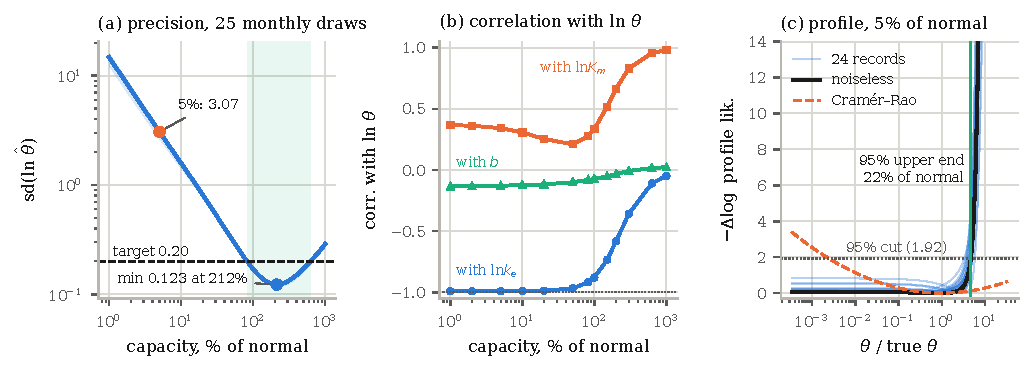
\includegraphics[width=\linewidth]{pi_t1.pdf}
\end{figure}

\subsection{Panel (a)} The horizontal axis is the patient's capacity as a percentage of normal,
from $1\%$ to $1000\%$ (logarithmic). The vertical axis is $\sdl{\hat\theta}$ (logarithmic).
The blue curve is the precision the design achieves; the dashed line is the target. Read it
like a map of where the design works: the curve is below the dashed line only inside the
green band, from $82\%$ to $627\%$ of normal. At $5\%$ (orange dot) it is $3.07$, fifteen
times the target.

\subsection{Panel (b)} This panel gives the reason. It shows how strongly the estimate of
$\theta$ is tied to each of the other unknowns. A value of $-1$ means a perfect trade-off: a
larger $\theta$ together with a smaller $k_e$ explains the data exactly as well. Follow the
blue line (``with $\ln k_e$''): below about $50\%$ of normal it sits at $-1$. In a severe
patient the enzyme removes only a small share of the metabolite ($16\%$ at $5\%$ of normal), so
the data cannot separate ``a bit more enzyme'' from ``a bit more of the other clearance
route''. The orange line rises at very high capacity, where a different trade-off (with $K_m$)
takes over; that is why the curve in panel (a) rises again on the right.

\subsection{Panel (c)} This is the most technical panel. The horizontal axis is a candidate
value of $\theta$ divided by the true value; the vertical axis says how much worse the data
fit becomes at that candidate ($0$ is the best fit). Candidates whose curve stays below the
dotted line at $1.92$ are compatible with the data at the $95\%$ level. Look at the black
curve: on the left it stays flat at zero all the way down to a thousandth of the truth, so
the data cannot rule out a patient with almost no enzyme; on the right it climbs steeply, so
the data \emph{can} rule out more than about $22\%$ of normal (green line). The dashed orange
parabola is what a well-behaved problem would look like; the real curve does not have that
shape.

\subsection{Take-away} At $5\%$ of normal the record supports a one-sided statement
(``capacity is below about $22\%$ of normal''), not a measurement.

\subsection{What it does not say} It does not say that capacity can never be measured: it
says this design, with these unknowns, cannot. Figure~3 asks whether other measurements help.

\section{Figure 2: the same failure as geometry}

\subsection{The question} Why exactly do the draws fail to pin down capacity?

\begin{figure}[h]
\centering
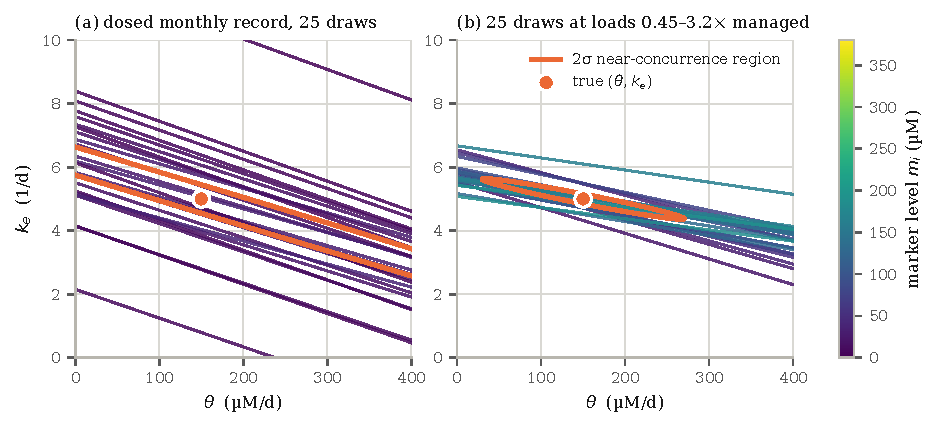
\includegraphics[width=0.92\linewidth]{pi_pencil.pdf}
\end{figure}

\subsection{What is drawn} Each blood draw gives one equation with two unknowns, capacity
$\theta$ (horizontal axis) and the other clearance route $k_e$ (vertical axis). One equation
with two unknowns is a \emph{line}: every point on it explains that draw exactly. Each
coloured line is one draw; the colour is the measured metabolite level (purple low, yellow
high). If there were no measurement noise, all lines would cross at the true value (orange
dot). The orange outline is the region where they nearly cross, that is, the uncertainty.

\subsection{How to read it} Think of it as triangulation. Each draw is a bearing towards an
unknown position. Bearings taken from very different directions cross sharply; bearings taken
from almost the same direction run nearly parallel, and the crossing point smears out along
them. The steepness of each line depends only on the metabolite level of that draw.

\subsection{Panel (a)} The real monthly record. The metabolite levels are all low and similar,
so all lines have nearly the same slope. They run almost parallel, and the region where they
nearly cross is a long thin sliver: capacity is unknown along the whole length of it.

\subsection{Panel (b)} A hypothetical record in which the dietary load is varied over a very
wide range. The high-metabolite draws (yellow) have different slopes, the lines now cross at
an angle, and the region shrinks to a small spot near the truth.

\subsection{Take-away} Precision needs draws at very different metabolite levels. In practice
those levels require loads far above what a severe patient tolerates (the parent model predicts
decompensation), so panel (b) is a picture of why the problem is hard, not a proposal.

\section{Figure 3: does any other measurement help?}

\subsection{The question} If we add other measurements to the blood record, does the precision
reach the target?

\begin{figure}[h]
\centering
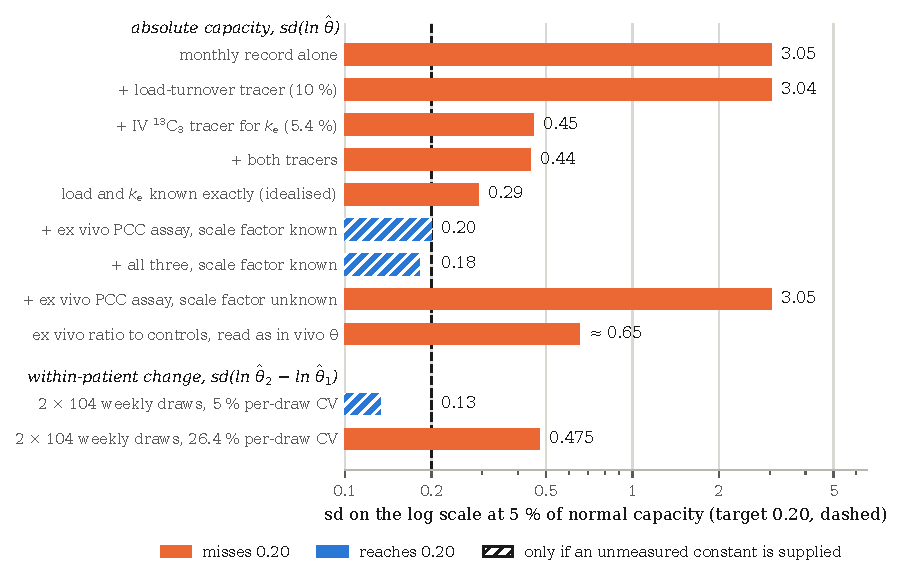
\includegraphics[width=0.8\linewidth]{pi_routes.pdf}
\end{figure}

\subsection{What is drawn} Each bar is one combination of measurements. Its length is the
precision it achieves, $\sdl{\hat\theta}$, on a logarithmic axis, so \emph{shorter is better}.
The dashed vertical line is the target $0.20$. Orange bars miss the target, blue bars reach it,
and hatched blue bars reach it only if an unmeasured constant is supplied (Section~1).

\subsection{How to read it, top group} Read the bars from the top as a story. The record
alone: $3.05$. Adding a tracer measurement of the load hardly helps ($3.04$). Adding a tracer
that measures the other clearance route $k_e$ helps a lot ($0.45$), and both together give
$0.44$, the best that available instruments achieve; still more than twice the target. Even
knowing those two perfectly leaves $0.29$. Only adding a direct reading of the enzyme (the ex
vivo assay on the patient's cells) reaches $0.20$, and that bar is hatched: it assumes we know
how test-tube activity in cells converts into whole-body capacity. The bar two rows further down
shows what happens without that conversion factor: $3.05$, no better than the record alone. The last
bar of the group tries to avoid the factor by comparing the patient's cells with healthy
controls; that removes the factor but measures test-tube activity rather than whole-body
capacity, and the gap between the two leaves about $0.65$.

\subsection{How to read it, bottom group} These two bars answer a different question: not
``what is this patient's capacity?'' but ``has it changed between two periods?''. Here the
unknown constants cancel, because they are the same in both periods, and the model gives
$0.13$, well below the target. It is hatched because it assumes the metabolite varies by only
about $5\%$ from one draw to the next in a stable patient, which has not been measured in
propionic acidaemia. The bar below uses the only published figure ($26.4\%$, for a related
marker in healthy adults) and gives $0.475$.

\subsection{Take-away} There is no solid blue bar in the top group. Every route to the
absolute level either misses the target or needs a constant nobody has measured. Change within
one patient is reachable, if the marker turns out to be stable enough.

\section{Figure 4: what the dosing interval needs}

\subsection{The question} Can the dosing interval be lengthened without knowing the patient's
capacity, and what does that depend on?

\begin{figure}[h]
\centering
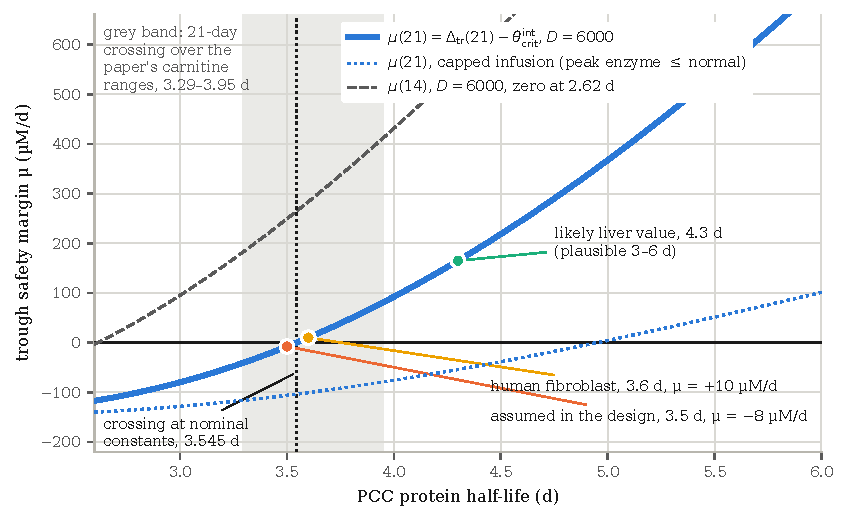
\includegraphics[width=0.78\linewidth]{pi_margin.pdf}
\end{figure}

\subsection{What is drawn} The horizontal axis is the PCC protein half-life: how long the
enzyme delivered by each dose lasts. A longer half-life leaves more enzyme at the low point
just before the next dose (the trough). The vertical axis is the safety margin of the most
vulnerable patient, one with no enzyme of their own: the enzyme left at the trough minus the
critical capacity below which the parent model loses its stable state. Above the horizontal
zero line the interval is safe for \emph{every} patient, without knowing anyone's capacity.
Below it, safety depends on the patient's own capacity, which Figures~1--3 show cannot be
measured.

\subsection{The curves} The thick blue curve is the 21-day interval at the booked dose; it
crosses zero at $3.545$ days. The grey dashed curve is the 14-day interval, which crosses zero
far to the left, at $2.62$ days. The dotted blue curve is the 21-day interval at the smaller
dose the paper considers the largest admissible in severe patients; it crosses zero much later,
at $4.39$ days. The grey band shows where the 21-day crossing could lie once the unmeasured
carnitine constants are allowed to vary ($3.29$ to $3.95$ days).

\subsection{The dots} Orange: the $3.5$ days assumed in the paper's design, just below zero.
Yellow: the only human measurement, $3.6$ days in skin cells, just above zero. Green: the likely
value in liver, about $4.3$ days, an estimate from comparable proteins rather than a
measurement.

\subsection{How to use it} Pick a half-life on the horizontal axis, go up to the curve for the
interval and dose you care about, and check whether you are above or below zero. Table~2 of the
note gives the same crossings as numbers, for all three intervals and both doses.

\subsection{Take-away} The interval decision does not need capacity; it needs the half-life
(and the dose). At the likely liver value of $4.3$ days, all three intervals are safe at the
booked dose; at the smaller admissible dose, the 21-day interval is not.

\subsection{What it does not say} ``Safe'' here means that the patient keeps a stable state at
their usual load, as the parent model defines it. It does not cover an intercurrent illness,
which raises the load, and it is not a clinical recommendation for an investigational drug.

\section{A short glossary}

\begin{description}[leftmargin=1.4em,style=nextline]
\item[$\theta$ (capacity)] the patient's residual PCC enzyme capacity; $5\%$ of normal is the
severe range.
\item[$k_e$] the strength of the other clearance route (conjugation to carnitine and renal
loss), which competes with the enzyme.
\item[Cram\'er--Rao bound] the best precision any unbiased estimate can achieve from a given
record; the note's precisions are of this kind, so real estimates can only be worse.
\item[Half-life] the time for half of the delivered enzyme to be broken down.
\item[Trough] the lowest level of delivered enzyme, just before the next dose.
\item[Critical capacity] the enzyme capacity below which the parent model has no stable
state at the given load.
\end{description}

\end{document}
